 \documentclass[15pt]{article}
\usepackage{geometry}
\usepackage{amsmath}
\usepackage{amssymb}
\usepackage{enumitem}
\usepackage{float}
\usepackage{fancyhdr}
\usepackage{tikz}
\usepackage{graphicx}
\usepackage{datetime}
\usepackage{fdsymbol}
\usepackage[utf8]{inputenc}
\usepackage{mathtools}
\usepackage[nottoc,numbib]{tocbibind} 
\DeclarePairedDelimiter\ceil{\lceil}{\rceil}
\DeclarePairedDelimiter\floor{\lfloor}{\rfloor}
\usepackage{listings}
\graphicspath{{Images/}}

\usetikzlibrary{trees}
\pagestyle{fancy}

\lhead{APS420H1S}
\chead{Technology, Engineering and Global Development}
\rhead{Assignment 1}

\lfoot{Jia Ming (Carter) Huang}
\rfoot{1003893245}

\begin{document}
\begin{center}
Jia Ming (Carter) Huang (Student ID: 1003893245)

%You don't need to modify the marking table.
\begin{table}[h]
\centering
\begin{tabular}{|l|l|l|l|l|l|l|l|l|l|l|}
\hline
     & Q1 & Q2 & Q3 & Q4 & Q5 & Q6 & Q7 & Total \\ \hline
Mark &    &    &    &    &    &    &    &       \\ \hline
\end{tabular}
\caption{Marking Table}
\end{table}

Due Date: Friday, February 11, 2022, 11:59 PM \\
\indent Number of Pages: 47
\end{center}

\noindent Please note that all the R code used to generate the data used in this analysis is included for your reference in Appendix A.

\renewcommand*\contentsname{List of Problems}

\tableofcontents

\newpage

\section{Correlation Between GDPPC and Geographical Location}

Since the end of the Second World War, terms such as "Third World" and "Global South" evolved in developed countries to impose an ideology that the world is clearly divided into rich and poor. "Global South" is a recent term that seeks to eliminate some of the derogatory contexts of the term "Third World". This investigation examines the emergence of the term "Global South" and its statistical implications. We must first define key terms that will aid in our investigation.
\\
\\ GDP per capita (GDPPC) is the measure of wealth by dividing the gross domestic product of a country equally among its population. While the purchasing power of US\$1 in Country $A$ may not reflect the purchasing power of US\$1 in Country $B$, this metric pegs the wealth of nations to the US dollar. Due to the abandonment of Britain's Gold Standard, the Bretton Woods Agreement, and America's role as a weapon's supplier in World War II, the Global Reserve Currency today is the United States Dollar \cite{1}, which serves as a reliable benchmark of economic wealth across nations. The term "Global South" implies that nations north of the equator are more wealthy in terms of GDP per capita. In TCdata360 \cite{2}, there are 67 high income countries (HICs), of which only 7 are in the Southern Hemisphere. \\
\\ Before we delve into our statistical analysis, it is important to note that only 13\% of the human population lives south of the equator \cite{3}, which is a major contributor to the distribution of wealth by geographic location. Intuitively, we recall that developed nations such as Australia and New Zealand are in the Southern hemisphere as well. This begs the question: does GDP per capita increase as latitude increases? \\
\\
Figures 1, 4, 7, and 10 show the distribution of GDP per capita versus latitude in 1960, 1980, 2000, and 2019, respectively. Notice that the orange dots per the Income Level legend are HICs. If an individual with the belief that the "Global South" is an accurate description of the state of economics of nations, they would appeal to their own confirmation biases that the data indeed proves the dependence of a country's economics on geographic location. As inquisitive data scientists, we extract the R-squared values from the data to see the strength of correlation between latitude and GDP per capita.\\
\\
Figures 2, 5, 8, and 11 show the correlation between GDP per capita versus latitude in 1960, 1980, 2000, and 2019, respectively. We can see that regardless of time, there is low correlation ($ <0.4$) between GDP per capita versus latitude, which suggests that the wealth of nations does not depend on latitude. Let us recall that in our earlier analysis, the Southern Hemisphere also hosts wealthy nation's like Australia and New Zealand, and that the concentration of HICs in the South are comparable to that of the North. In the South, $7/67 \approx 10\%$ of HICs are shared by $\approx 13\%$ of the Earth's population. This prompts us to look at the question differently. One hypothesis is that nations further from the equator are wealthier, because harsher climates promote the development of technology \cite{4}. Technology, being a driving force of economic development and superiority is a common denominator between developed countries far from the equator. Could we look at the distance from the equator as an indicator of economic success? \\
\\
Figures 3, 6, 9, and 12 show the correlation between GDP per capita versus distance from the equator in 1960, 1980, 2000, and 2019, respectively. In Figure 3, we see that the correlation between distance from the equator and GDP per capita in 1960 is $\approx 0.42$, which is the highest linear regression R-squared value in all comparisons. Coupled with high p-values in our regression coefficients, we can conclude that there is not a significant correlation between the geographic location and economic well-being of a country. \\
\\
Our analysis doesn't stop here. As we analyze the trends over time, from 1960 to 2019, we notice that the correlation between the geographic location and economic well-being of countries decreased significantly. If we fancied the hypothesis that geographically extreme countries have better economic well-being, we can conclude that in 1960, there was an acceptable correlation that countries far from the equator were in fact richer. If we take into consideration the population distribution between north and south, and neglect the data from the southern hemisphere, the term "Global South" may have been sensible. However, as the correlation wanes today, partly due to the rising economies and populations of nation's near the equator such as China, India, and Nigeria, this term is no longer an accurate description of the world's economic affairs. We can see that the "Global North" is a term that includes North America, Europe, Australia and New Zealand, which is more on par with the observation that the correlation between GDP per capita and distance from the equator is stronger than that of absolute latitude.\\
\\
Therefore, through statistical analysis and an understanding of geopolitical situations that gave rise to terms like "Third World" and "Global South", we realize that the surface-level trends we see in our Latitude versus GDP per capita graphs over time only paint a biased view towards the economic state of the world. There are simply more people, borders, and as a result, conflicts near the equator. The Western World is a direct beneficiary of the consequences of twentieth century conflicts preceded by an era of colonialism. The geographic location of developed nations today is merely a coincidence for their economic well-being. Rather, geographic location may be a catalyst for sociopolitical, cultural, and economic forces that bring about strong economic performance in the modern era. Instead of using the term "Global South", which is quite inaccurate, we should use the term "Developing Nations". Since there is no direct, statistically significant correlation between geography and a country's economic well-being, its preferable to describe a nation by its rate of economic growth. This is a direct, unbiased, value-free, and statistically perfect indicator of economic well-being, as it is a one-to-one comparison between GDP per capita and GDP per capita growth.

\begin{figure}[H]
    \centering
    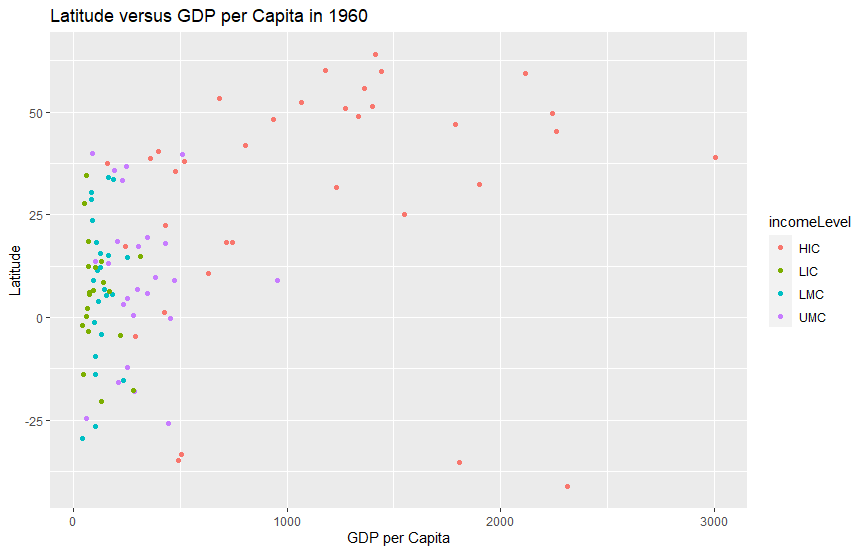
\includegraphics[scale = 0.5]{Part1_1960.png}
    \caption{Latitude versus GDP per Capita in 1960}
\end{figure}

\begin{figure}[H]
    \centering
    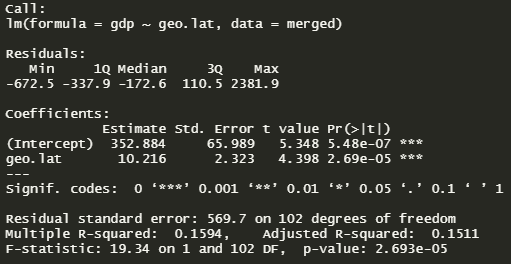
\includegraphics[scale = 0.5]{Part1_latitude_r^2_1960.PNG}
    \caption{Statistical Correlation by Latitude in 1960}
\end{figure}

\begin{figure}[H]
    \centering
    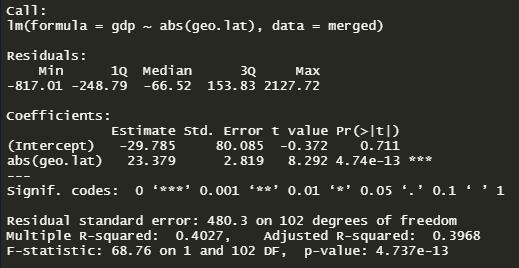
\includegraphics[scale = 0.5]{Part1_dist_from_equator_r^2_1960.PNG}
    \caption{Statistical Correlation by Distance From Equator in 1960}
\end{figure}

\begin{figure}[H]
    \centering
    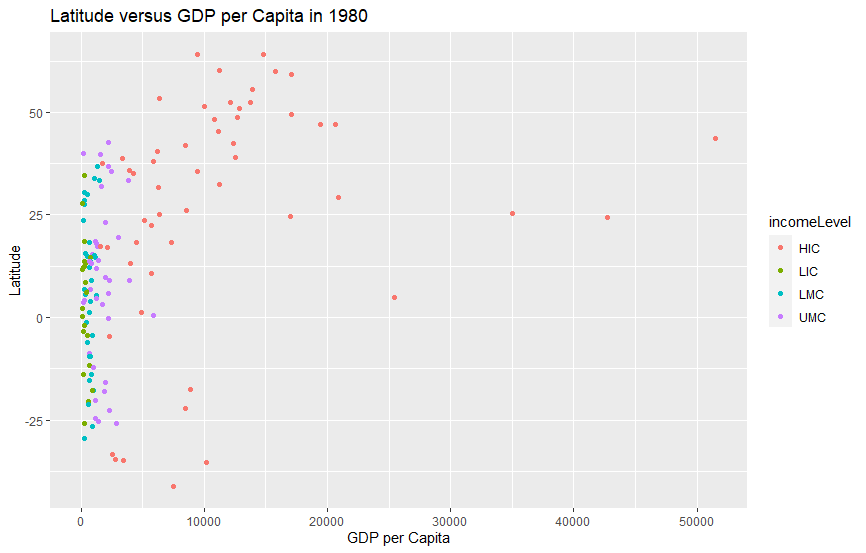
\includegraphics[scale = 0.5]{Part1_1980.png}
    \caption{Latitude versus GDP per Capita in 1980}
\end{figure}

\begin{figure}[H]
    \centering
    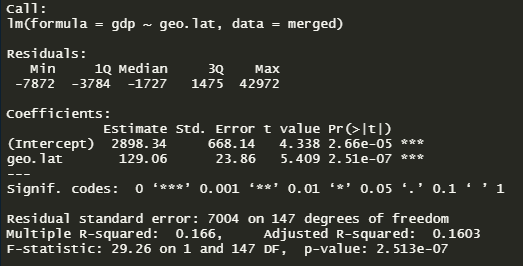
\includegraphics[scale = 0.5]{Part1_latitude_r^2_1980.PNG}
    \caption{Statistical Correlation by Latitude in 1980}
\end{figure}

\begin{figure}[H]
    \centering
    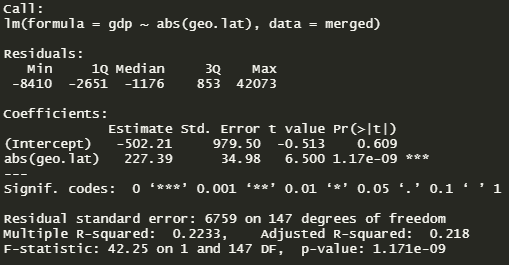
\includegraphics[scale = 0.5]{Part1_dist_from_equator_r^2_1980.PNG}
    \caption{Statistical Correlation by Distance From Equator in 1980}
\end{figure}

\begin{figure}[H]
    \centering
    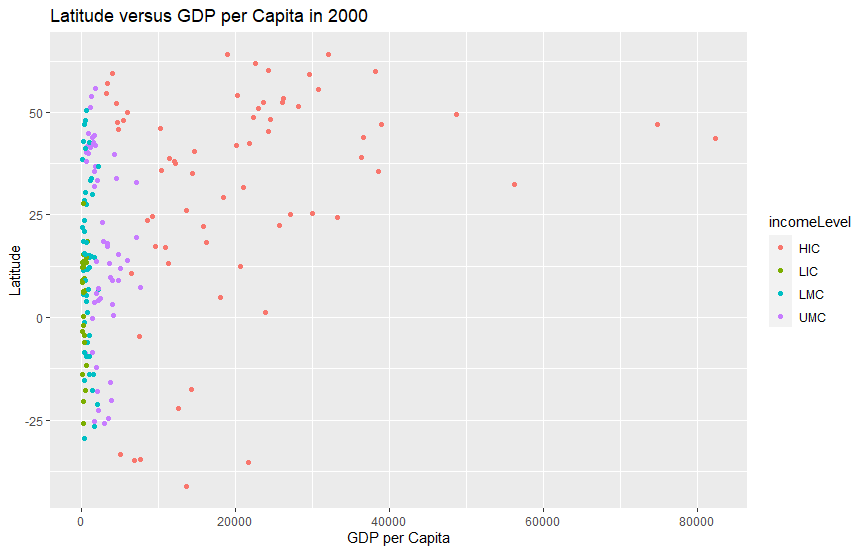
\includegraphics[scale = 0.5]{Part1_2000.png}
    \caption{Latitude versus GDP per Capita in 2000}
\end{figure}

\begin{figure}[H]
    \centering
    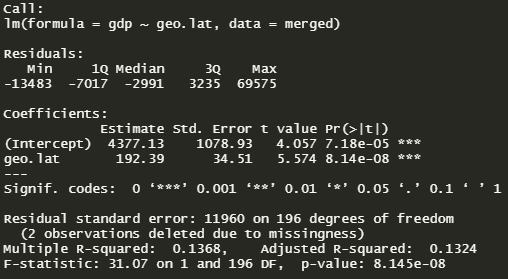
\includegraphics[scale = 0.5]{Part1_latitude_r^2_2000.PNG}
    \caption{Statistical Correlation by Latitude in 2000}
\end{figure}

\begin{figure}[H]
    \centering
    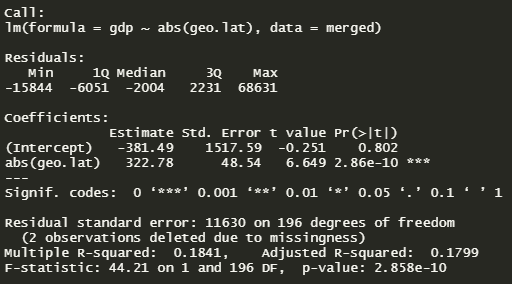
\includegraphics[scale = 0.5]{Part1_dist_from_equator_r^2_2000.PNG}
    \caption{Statistical Correlation by Distance From Equator in 2000}
\end{figure}

\begin{figure}[H]
    \centering
    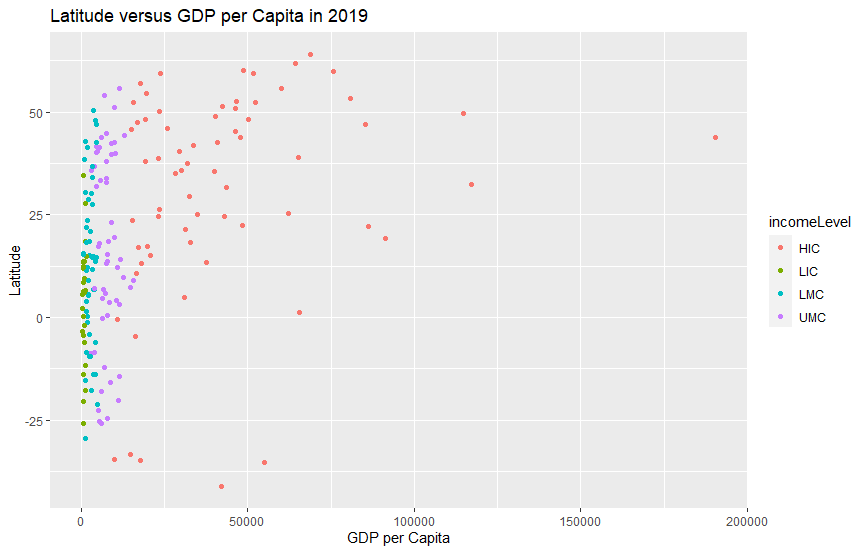
\includegraphics[scale = 0.5]{Part1_2019.png}
    \caption{Latitude versus GDP per Capita in 2019}
\end{figure}

\begin{figure}[H]
    \centering
    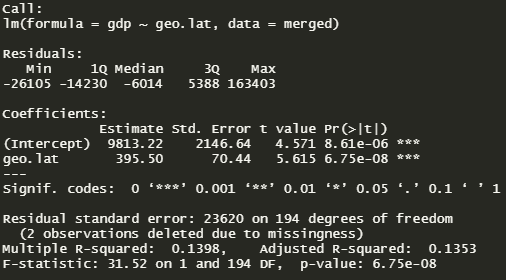
\includegraphics[scale = 0.5]{Part1_latitude_r^2_2019.PNG}
    \caption{Statistical Correlation by Latitude in 2019}
\end{figure}

\begin{figure}[H]
    \centering
    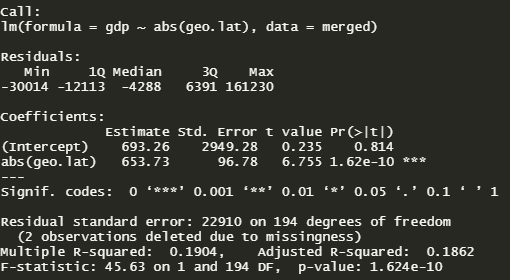
\includegraphics[scale = 0.5]{Part1_dist_from_equator_r^2_2019.PNG}
    \caption{Statistical Correlation by Distance From Equator in 2019}
\end{figure}

\newpage

\section{Fixed Broadband Internet Subscriptions in Landlocked Developing Country's (LLDCs)}

In Figure 13, we can see that the Fixed Broadband Internet Subscriptions in Non-LLDCs are higher than in LLDCs between 2017 and 2018. The box plot medians can be used to analyze statistical significance \cite{5}. If we remove the outlier in the LLDC box plot, we can see that its median is lined up with the bottom of the Non-LLDC box plot. This suggests that there is marginally statistical difference between the two, and that it is marginally likely for LLDCs and Non-LLDCs to have statistically significant disparities between the number of Fixed Broadband Internet Subscriptions. However, while both medians are on the lower side of the Fixed Broadband Internet Subscriptions, we can see that in both cases of LLDCs and Non-LLDCs, there is heavy variance towards the higher end of the number of Fixed Broadband Internet Subscriptions, which suggests an internet access inequality around the globe.

\begin{figure}[H]
    \centering
    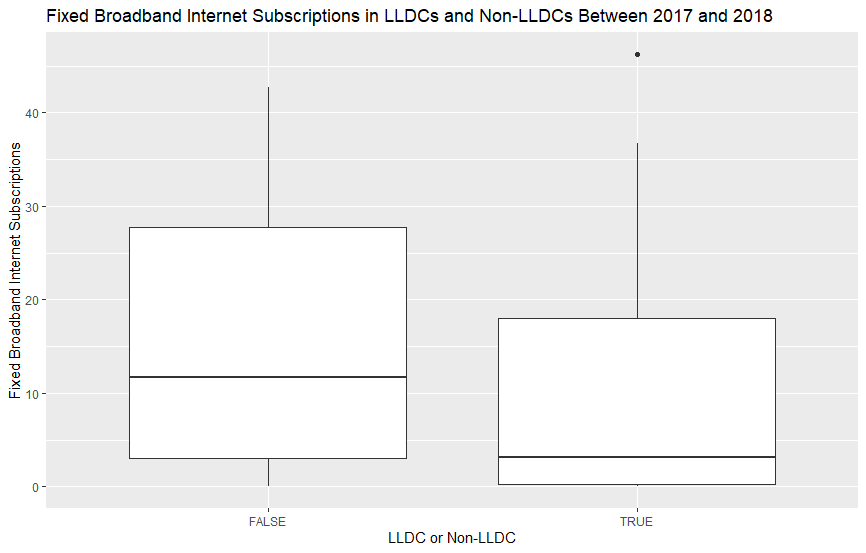
\includegraphics[scale = 0.7]{Part2_box.png}
    \caption{Fixed Broadband Internet Subscriptions in LLDCs and Non-LLDCs Between 2017 and 2018}
\end{figure}

\noindent As we analyze the data across time in Figure 14, we see that between 2007 and 2018, both LLDCs and Non-LLDCs experienced significant growth in the number of Fixed Broadband Internet Subscriptions. However, the overall trend seems to suggest that LLDCs are experiencing less growth overall, and the disparity is growing. \\
\\
While LLDCs are able to gain internet access, they don't have landing sites for the submarine cables that connect the world to the network \cite{6}. Without access to the ocean, LLDCs gain internet access by connecting to landlines in neighbouring nations that have access to the ocean. However, this poses two challenges: LLDCs have to share the same internet infrastructure with other countries, which can disconnect the service due to dispute or necessity \cite{6}. Furthermore, in order for internet to reach landlocked countries, they must build cables across land, which can have difficult terrain. This significantly increases the cost of delivering internet to LLDCs, which raises the cost of internet access for countries already disadvantaged economically due to their geography. Considering that the Internet is responsible for a sizeable portion of the world's economic growth, poor access to Internet is detrimental to LLDCs. Consider that in Yemen, a 5GB movie takes 30 hours to download, while in Taiwan, it takes just 8 minutes \cite{7}. Although Yemen is not an LLDC, the situation highlights how slow internet access can significantly reduce efficiency and in turn, economic growth.\\
\\
To address the issue of internet cable access in LLDCs, there can be international provisions in place to guarantee access to the ocean. For example, land which internet delivery cables sits on can be considered international territory, and only cables originating from these central delivery lines can serve as a country's sovereign property. This ensures that each country is able to access the Internet fairly, while also maintaining their own infrastructure so as not to do so at the expense of others. This solves the political pressure for nation's to maintain good relations in order to have reliable internet access. Furthermore, in the short term, LLDCs can try to build relations with other Non-LLDCs that they share borders with to provide redundant access to internet in case of disputes. To address the issue of bandwidth, speed, and penetration, new technologies that don't rely on cables can provide sustainable internet to LLDCs. LLDCs can focus on satellite networks that can transmit internet from offshore locations, where they can hook up to the global internet supply. Investing in wireless infrastructure can eliminate the burdens of internet access in LLDCs, so long as wireless technology can be just as reliable as broadband.

\begin{figure}[H]
    \centering
    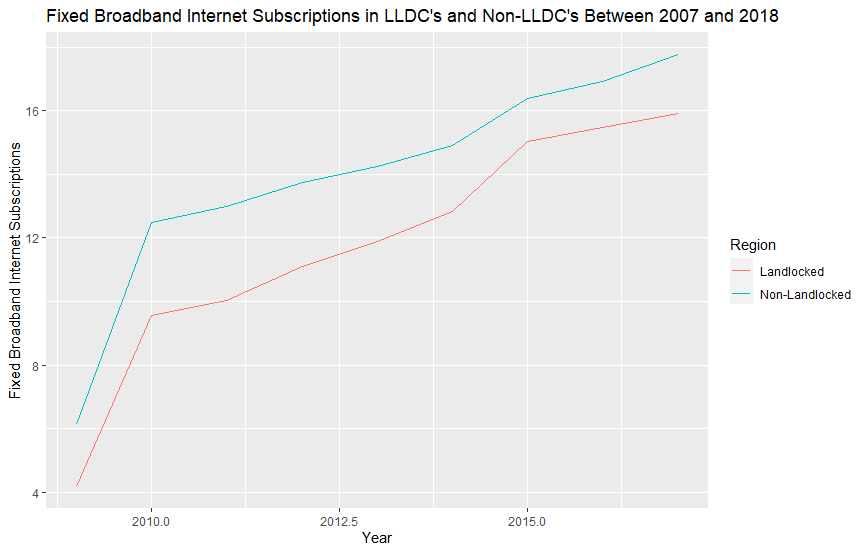
\includegraphics[scale = 0.7]{Part2_Growth.png}
    \caption{Fixed Broadband Internet Subscriptions in LLDCs and Non-LLDCs Between 2007 and 2018}
\end{figure}

\newpage

\section{Life Expectancy}

Life expectancy has grown significantly since 1960 as a result of technological advancements and the absence of wars of attrition. First, we must discuss how we gather, sanitize, and interpret the life expectancy data. By taking the TCdata360 datasets \cite{2} for life expectancy at birth of males and females from 1960 to 2019, we calculate the cell-by-cell average for each country, each year. Then, we loop through each row and column and take the change in life expectancy for each consecutive year in each country. Finally, we keep track of the maximum and minimum life expectancy at birth, as well as the year that these changes occurred for each nation to gain insight into socioeconomic factors that caused these changes.\\
\\
Cambodia and Rwanda had the largest increases in life expectancy, respectively. Cambodia's life expectancy at birth increased by 5.72 years from 33.51 to 39.23 between 1981 and 1982. Rwanda's life expectancy at birth increased by 4.45 years from 35.38 to 39.83 between 1996 and 1997.\\
\\
Not surprisingly, Rwanda and Cambodia had the largest decreases in life expectancy, respectively. Rwanda's life expectancy at birth decreased by 5.02 years from 38.46 to 33.44 between 1989 and 1990. Cambodia's life expectancy at birth decreased by 4.55 years from 32.88 to 28.33 between 1973 and 1974. In fact, in 1993, Rwanda's life expectancy at birth was only 26.20 years old, and in 1977, Cambodia's life expectancy at birth was only 19.34 years old. In comparison, countries like Japan and Iceland had life expectancy at birth in the high 70's during this timeframe.\\
\\
In Figure 15, we can see the life expectancy at birth of Cambodia and Rwanda. Let us research what happened in these two countries that caused such a massive fluctuation. In Cambodia, the Khmer Rouge began its insurgency in 1968, which overthrew Sihanouk, the head of state of Cambodia. In 1970, North Vietnam and the Khmer Rouge began the Cambodian Civil War. Between 1970 and 1975, between 600000 and 1000000 civil war deaths were recorded, with higher disputed figures as well \cite{8}. Between 1969 and 1973, the US bombed Cambodia, leading to between 30000 and 500000 deaths, which account for approximately 17\% of all civil war deaths \cite{8}. Furthermore, between 1975 and 1979, the Cambodian Genocide by the Khmer Rouge killed between 1.5 and 2 million people, which accounted for a quarter of Cambodia's population \cite{9}. Finally, to top it off, the Vietnamese invaded Cambodia in 1979 to destablize the Khmer Rouge regime \cite{8}. Therefore, as civilian deaths were rampant, and the nation was in abject poverty, Cambodia's life expectancy at birth sharply declined between 1970 and 1980.\\
\\
In the 1300s, the Tutsi people migrated into modern-day Rwanda, which was originally inhabited by the Twa and Hutu peoples. Tutsi's establish a kingdom that lasts over 500 years, until European forces occupy the nation. When Belgium retreated out of Rwanda in the 1950s, the Hutu people issued a manifesto calling for a change in Rwandan power structure, which formed Hutu political parties. Inter-ethnic violence due to historical Tutsi power and oppression lead to civil unrest that extends into the 1980s \cite{10}. In 1990, these ethnic clashes become the prelude to the Rwandan Civil War. At the end of the civil war, in 1994, the Hutu's commit genocide against the Tutsi people, resulting in between 400000 and 800000 deaths in just 100 days \cite{10}. Therefore, the constant ethnic conflicts in the mid-20th century in Rwanda, which sometimes resulted in as many as 20000 deaths in one instance \cite{10}, directly contributed to the sharp decline in Rwanda's life expectancy at birth between 1985 and 1994. \\
\\
Now, we take the gender-averaged mean life expectancy at birth of countries in Sub-Saharan Africa compared to the World, as shown in Figure 16. Life expectancy at birth in 1960 is significantly lower in Sub-Saharan Africa than in the rest of the world. Between 1990 and 2000, it seemed to drop slightly, before increasing at an accelerated rate. Note that the life expectancy at birth of the world includes Sub-Saharan Africa, so you can see a slight dip at the same time Sub-Saharan Africa experienced its plateau. Similarly, we can see that while Sub-Saharan Africa is experiencing significant life expectancy growth rates recently, the World's life expectancy is growing more slowly, despite inheriting the growth rate from Sub-Saharan Africa. This suggests that Sub-Saharan Africa's life expectancy growth rate is significantly higher than the rest of the world.\\
\\
Research shows that the dip in life expectancy in Sub-Saharan Africa in the 1990s was due to the HIV/AIDS epidemic \cite{11}. In contrast, the recent advancements in vaccinations and medical technology has reduced mortality by protecting against diseases like malaria. The growth in GDP per capita has also been significant, from \$600 in 2000 to more than \$1500 today, which explains the sharp increase in life expectancy in the 21st century. Furthermore, water quality and food nutrition has increased in Sub-Saharan Africa, allowing the middle-class to prosper and drive up life expectancy \cite{12}. These advancements are partly due to policy changes which open Africa up to investment around the world, like with the Belt and Road Initiative \cite{13}. 

\begin{figure}[H]
    \centering
    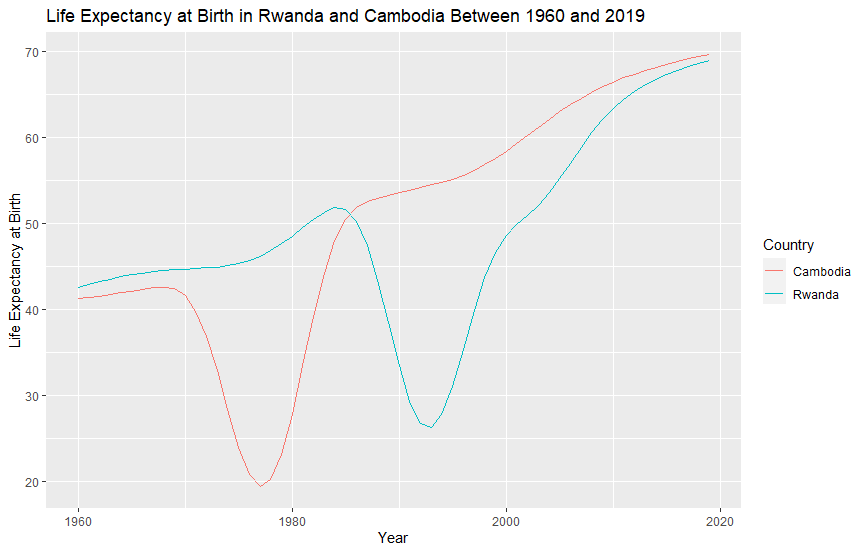
\includegraphics[scale = 0.7]{Part3_Rwanda_Cambodia.png}
    \caption{Life Expectancy at Birth in Rwanda and Cambodia Between 1960 and 2019}
\end{figure}

\begin{figure}[H]
    \centering
    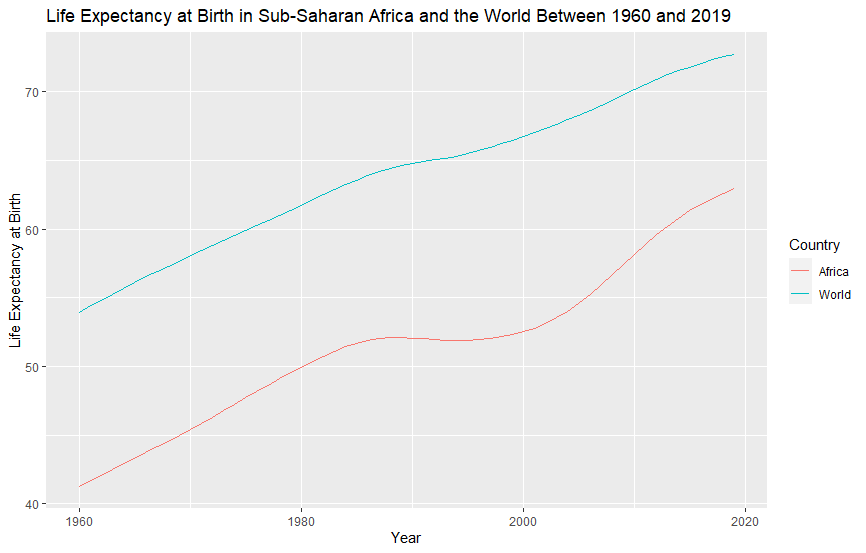
\includegraphics[scale = 0.7]{Part3_Africa.png}
    \caption{Life Expectancy at Birth in Sub-Saharan Africa and the World Between 1960 and 2019}
\end{figure}

\newpage

\section{Wealth-Health, Chicken-Egg}

In order to extend our analysis of life expectancy rates, let us take a look at Figures 17 and 18, which show Bangladesh, Korea, and Malaysia's life expectancy and GDP per capita, respectively. If we compare the growth of life expectancy  at birth, we can see that all three countries exhibit rather uniform growth from 1960 to 2019. On the other hand, the GDP per capita of all three nations are negligibly low between 1960 and 1980, before experiencing sharper growth until 2019. This suggests that nation's get healthier regardless of wealth, and wealth tends to follow after health. In fact, in Bangladesh, we can see that while life expectancy had been steadily growing from 1960 to 2019, the GDP per capita remains low compared to Korea and Malaysia. One hypothesis is that better health and higher life expectancy means more time for an individual to generate wealth. Let us do some research to explore this trend in more detail.\\
\\
First, we take a look at data during the COVID-19 pandemic, where the standardized deaths due to the virus is correlated with negative GDP growth \cite{14}. This implies that the decrease in health leads to the decrease in GDP, rather than the other way around. The reason is that before the pandemic, the global GDP was rising, and only took a downturn when the pandemic hit. Secondly, we take a look at the Preston Curve in 2012, which shows the relationship between wealth and health weakens as countries become wealthier. In fact, past a certain threshold, we see that higher income means lower life expectancy, and for developed countries, wealth and health are generally insignificantly correlated \cite{15}. In certain countries like Cuba and the Dominican Republic, life expectancy at birth is on par with countries like the US and Slovakia, respectively, despite having a significantly lower GDP per Capita \cite{15}. One explanation for this phenomenon is that health spending in emerging economies, while lower, has a comparatively significant impact than that in a developed nation. This is because the health infrastructure is so basic, that any spending in health will create a sizeable impact. Therefore, it is easier for the health of developing nations to improve without significant economic gains. However, while it seems like health comes before wealth, it is also proper to state that the correlation between the two are statistically insignificant, and there may not be a definitive cause and effect.\\
\\
In short, a higher standard of health is often accompanied by other factors, such as institutionalization, political stability, and access to clean water and sanitary services. These factors are also direct contributors to economic growth. In developing nations, the impact of health spending is more pronounced than in developed nations, so it is economically prudent for these nations to invest in health. Across a certain threshold, notably that of a developed nation, the relationship between health and wealth becomes insignificant. In emerging economies, we can say that there is some indication that health comes before wealth, but that this relationship depends on other factors which have statistically stronger correlations.

\begin{figure}[H]
    \centering
    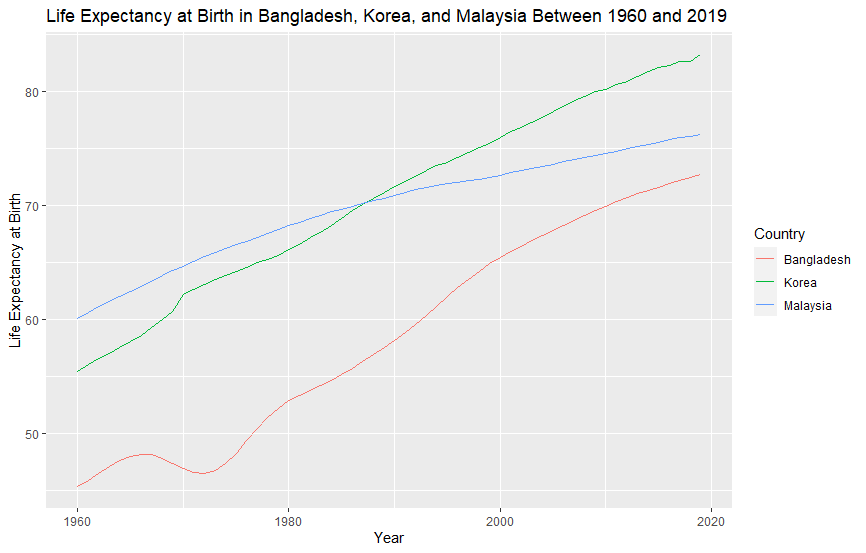
\includegraphics[scale = 0.7]{Part4_Life.png}
    \caption{Life Expectancy at Birth in Bangladesh, Korea, and Malaysia Between 1960 and 2019}
\end{figure}

\begin{figure}[H]
    \centering
    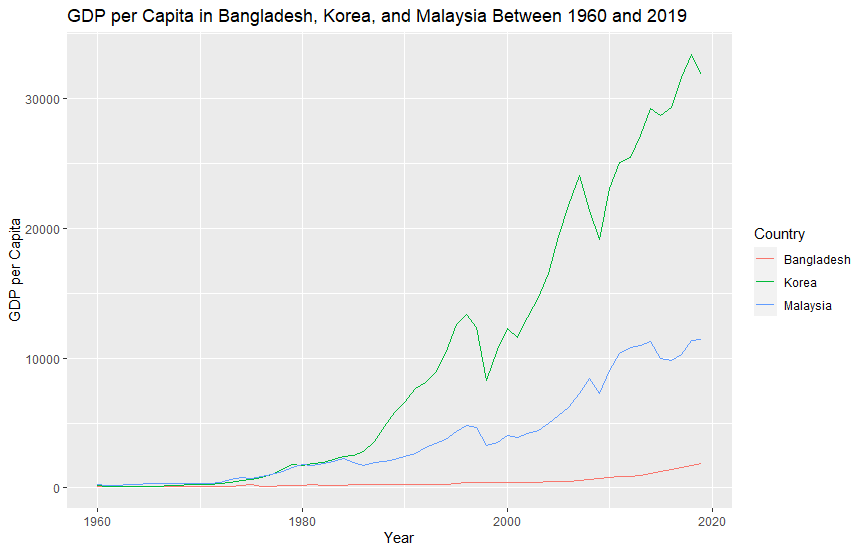
\includegraphics[scale = 0.7]{Part4_GDP.png}
    \caption{GDP per Capita in Bangladesh, Korea, and Malaysia Between 1960 and 2019}
\end{figure}

\newpage

\section{Socioeconomic Conditions That Affect a Nation's GII}

There are four socioeconomic factors that affect a country's innovation capacity and success. These are political stability, institutions, ease of getting credit, and entrepreneurship as a desirable career choice. In Week 2, class discussions referred to the lack of some of these factors as directly contributing to poverty \cite{16}, and in effect, a nation's Global Innovation Index (GII). First, we describe how and why each of these 4 factors influence a country's capacity to innovate.\\
\\
Political stability is defined by government transparency, predictability, and accountability \cite{17}. The more stable a nation is, the lower the risk to start a business and engage in entrepreneurial activity. Healthy economies are driven by market forces, rather than centralized economic planning, especially for entrepreneurs who are most at risk for policy changes and regulations. Therefore, it is intuitive to associate political stability with a capacity for innovation. We assess this relationship in Figures 19 and 20.\\
\\
The institutional framework of a nation is also important in assessing the capacity for innovation. Nations with strong institutional frameworks offer many protections for businesses, so that there is predictable and accountable support from public services. Innovation occurs in low-risk settings, so the peace of mind offered by strong institutional frameworks will undoubtedly promote innovation capacity. We assess this relationship in Figures 21 and 22.\\
\\
Investment is the primary method of raising capital for new businesses \cite{18}. Innovation can only persist if businesses are able to raise capital to run daily business operations. Credit is a way for financial institutions to lend money to business owners while assessing risk. The ease of getting credit is directly related to the ease of raising capital. Therefore, it is imperative for businesses to obtain the economic foundations required to continue operations before innovation can occur. We assess this relationship in Figures 23 and 24.\\
\\
Entrepreneurship is the fundamental pillar of innovation, because it allows new business owners to bring their ideas into practice. Entrepreneurship as a desirable career choice pushes more individuals to start businesses, rather than to work at corporate settings. This encourages free market competition, as new ideas are being injected into the market, rather than large corporations monopolizing goods and services. As we know, monopolies hinder innovation, because there are no longer disruptive forces to pressure businesses to improve their products \cite{19}. Therefore, entrepreneurship as a desirable career choice will ensure innovation capacity in a nation. We assess this relationship in Figures 25 and 26.\\
\\
Evidently, Institutions versus GII Index in 2020 shows a significant statistical correlation, with an R-squared value of 0.7617. This suggests that institutional foundations are the primary driver of a nation's innovative capacity and success. Furthermore, if we take a look at Figures 27 and 28, we can see that this same pattern and high correlation exists when we compare Institutions with GDP per Capita across the world. It becomes easy to see that as the Institutions Index increases, so does the wealth of the nation. The conclusion we can draw is that institutionalization builds innovation, and as a result, wealth.

\begin{figure}[H]
    \centering
    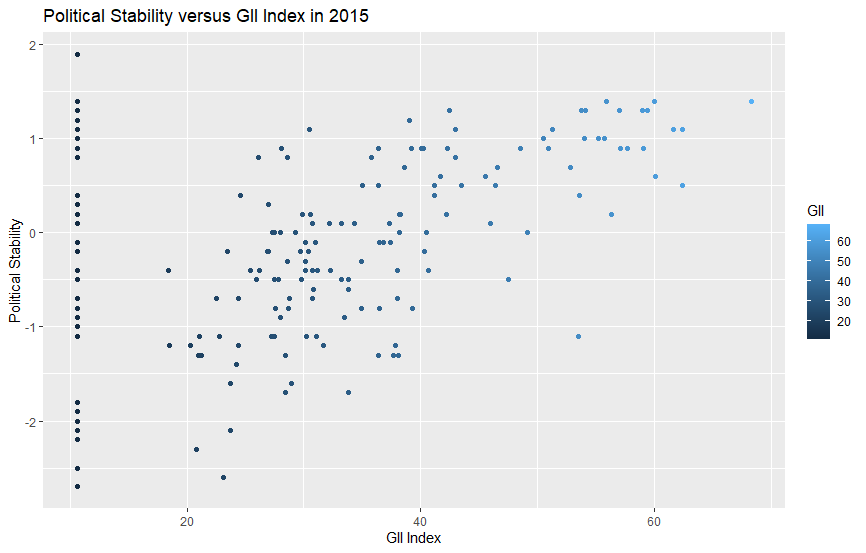
\includegraphics[scale = 0.7]{Part5_Political.png}
    \caption{Political Stability versus GII Index in 2015}
\end{figure}

\begin{figure}[H]
    \centering
    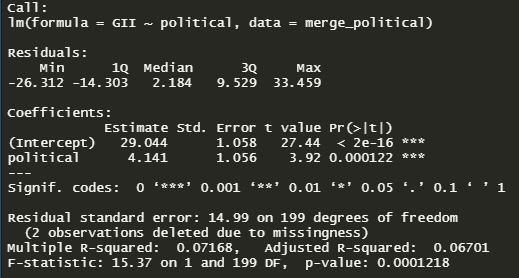
\includegraphics[scale = 0.7]{Part5_Political_r^2.png}
    \caption{Statistical Correlation by Political Stability in 2015}
\end{figure}

\begin{figure}[H]
    \centering
    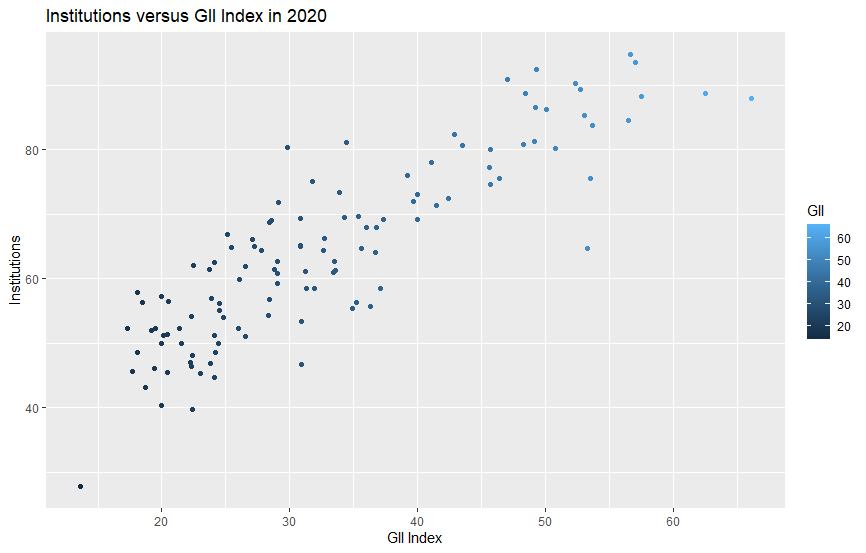
\includegraphics[scale = 0.7]{Part5_Institutions.png}
    \caption{Institutions versus GII Index in 2020}
\end{figure}

\begin{figure}[H]
    \centering
    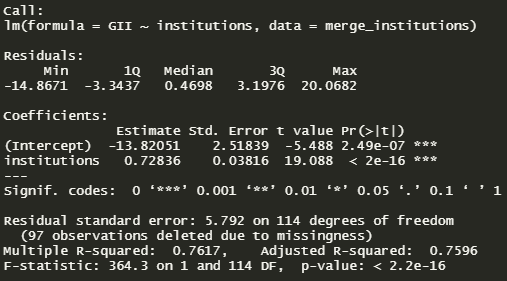
\includegraphics[scale = 0.7]{Part5_Institutions_r^2.PNG}
    \caption{Statistical Correlation by Institutions in 2020}
\end{figure}

\begin{figure}[H]
    \centering
    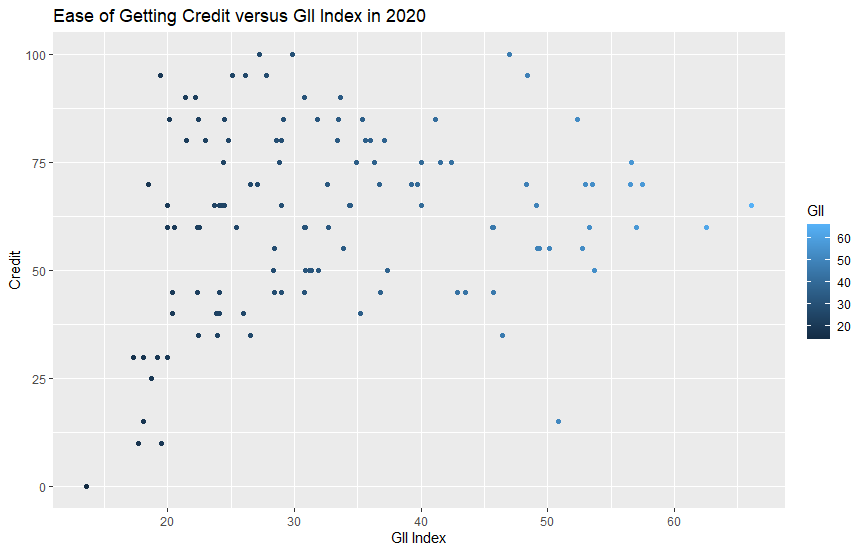
\includegraphics[scale = 0.7]{Part5_Credit.png}
    \caption{Ease of Getting Credit versus GII Index in 2020}
\end{figure}

\begin{figure}[H]
    \centering
    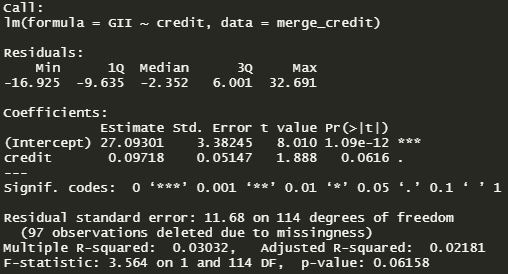
\includegraphics[scale = 0.7]{Part5_Credit_r^2.PNG}
    \caption{Statistical Correlation by Ease of Getting Credit in 2020}
\end{figure}

\begin{figure}[H]
    \centering
    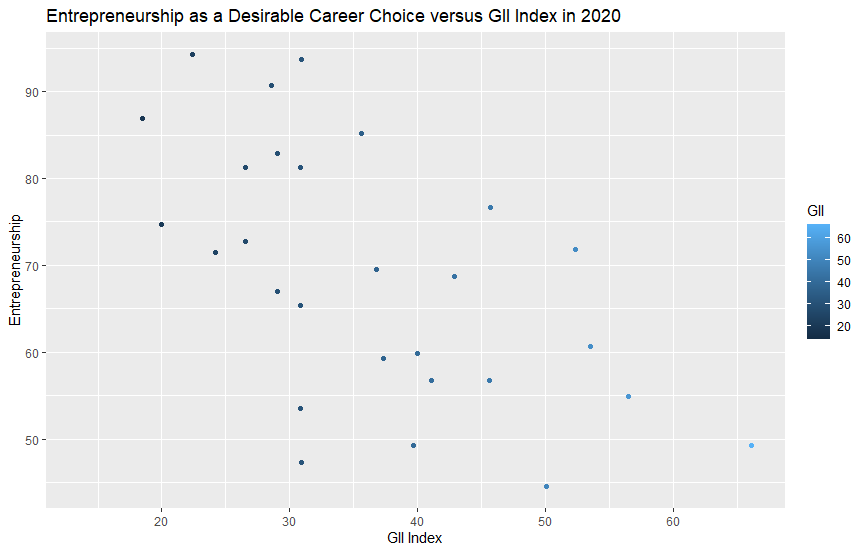
\includegraphics[scale = 0.7]{Part5_Entrepreneurship.png}
    \caption{Entrepreneurship as a Desirable Career Choice versus GII Index in 2020}
\end{figure}

\begin{figure}[H]
    \centering
    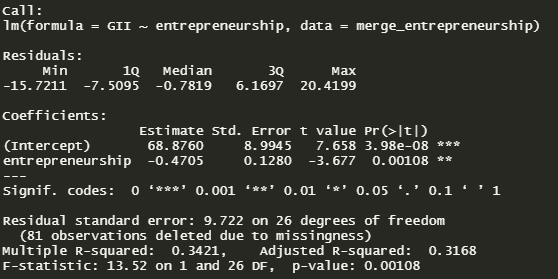
\includegraphics[scale = 0.7]{Part5_Entrepreneurship_r^2.PNG}
    \caption{Statistical Correlation by Entrepreneurship as a Desirable Career Choice in 2020}
\end{figure}

\begin{figure}[H]
    \centering
    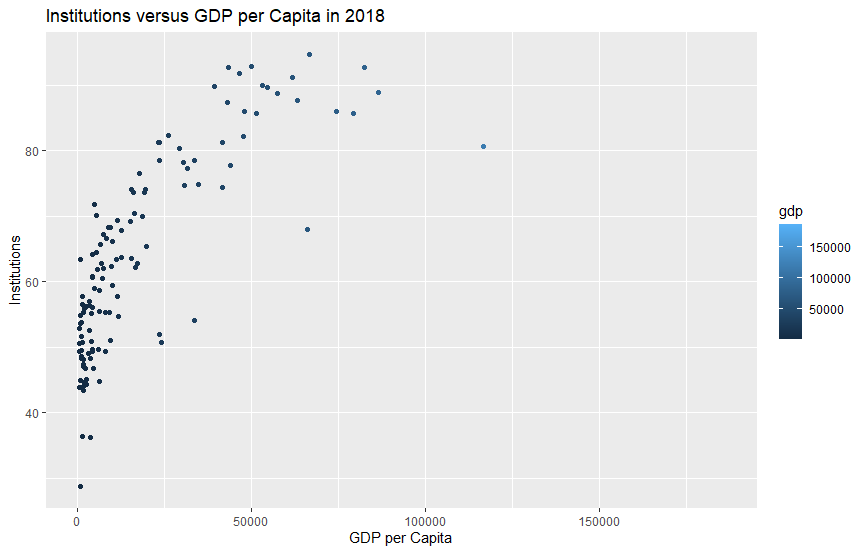
\includegraphics[scale = 0.7]{Part5_Institutions_GDP.png}
    \caption{Institutions versus GDP per Capita in 2018}
\end{figure}

\begin{figure}[H]
    \centering
    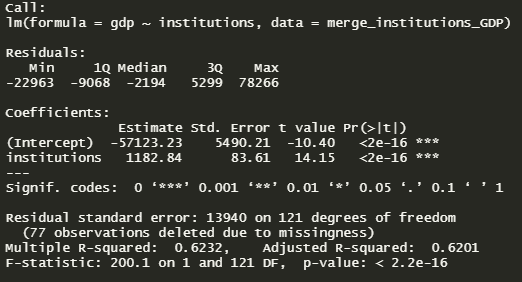
\includegraphics[scale = 0.7]{Part5_Institutions_GDP_r^2.PNG}
    \caption{Statistical Correlation by Institutions in 2018}
\end{figure}

\begin{figure}[H]
    \centering
    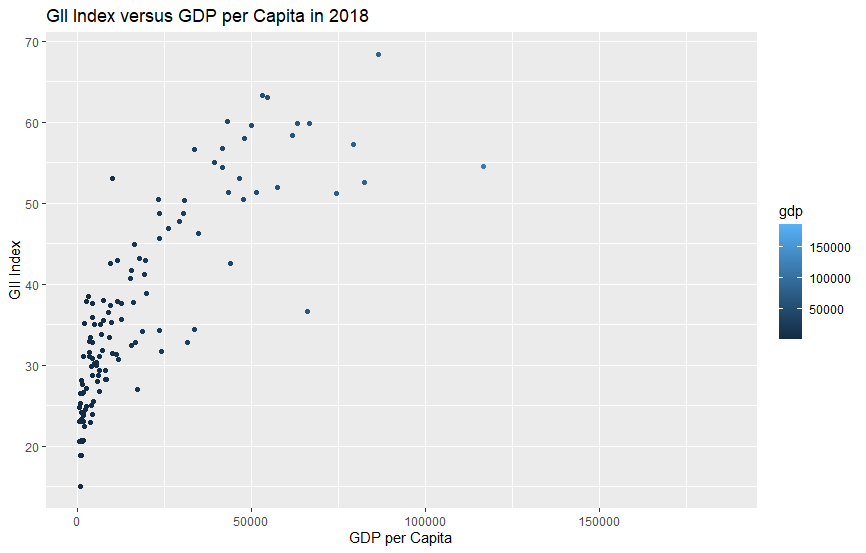
\includegraphics[scale = 0.7]{Part5_GII_GDP.png}
    \caption{GII Index versus GDP per Capita in 2018}
\end{figure}

\begin{figure}[H]
    \centering
    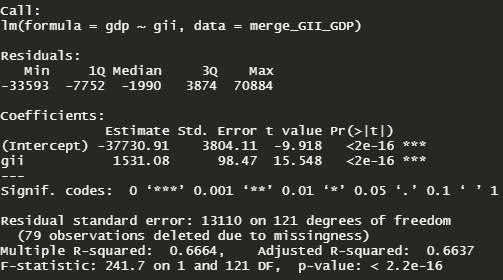
\includegraphics[scale = 0.7]{Part5_GII_GDP_r^2.PNG}
    \caption{Statistical Correlation by GII Index in 2018}
\end{figure}

\noindent As a remark, we may wish to consider why institution, and not the other three factors? In terms of entrepreneurship, although entrepreneurship does promote innovation, it may also be a fall-back for people who are unable to find a job due to a lack of talent or opportunity. In terms of ease of getting credit, it is dangerous for banks to lend credit out to anyone, anywhere. This was the primary catalyst for the US stock market crash of 1929 \cite{20}. Finally, political stability is an interesting one. Although the R-squared value is low, it may have been due to the cluster of countries with a low GII index scattered across the political stability spectrum. In fact, the p-value is quite low, which suggests that political stability does promote innovation. However, institutionalization is likely the primary driver of innovation capacity, because it signifies a mature government framework. This framework, understandably, showcases political stability and ease of getting credit in an accountable and predictable way. In fact, entrepreneurs arising from institutionalized countries are often driven and well-educated, rather than becoming entrepreneurs as a necessity for survival, as is often seen in low-income countries. The mingling of these four factors are key indicators for a country's innovative capacity and success; as we can further derive from Figures 29 and 30, where we see how a nation's GII is correlated strongly with it's GDP per capita.

\newpage

\section{Availability of Scientists and Engineers Around the World}

Intuitively, the more scientists and engineers there are in a country, the faster its technological development, and in turn, the better its economic well-being. Let us take a look at Figures 31 and 32, which show the distribution of scientists and engineers, and GDP per capita around the world, respectively. Immediately, we can see countries like Canada and India have a high number of scientists and engineers, but a lower GDP per capita than counterparts like the USA and Australia, which have comparatively less scientists and engineers. On the other hand, nations like China have less scientists and engineers, with a strong economy. It is important to note that the availability of scientists and engineers is not an absolute value, but rather, it is relative to the population of each country. This can be interpreted as a "per capita" concentration of scientists and engineers for the purpose of this analysis.
\\
\begin{figure}[H]
    \centering
    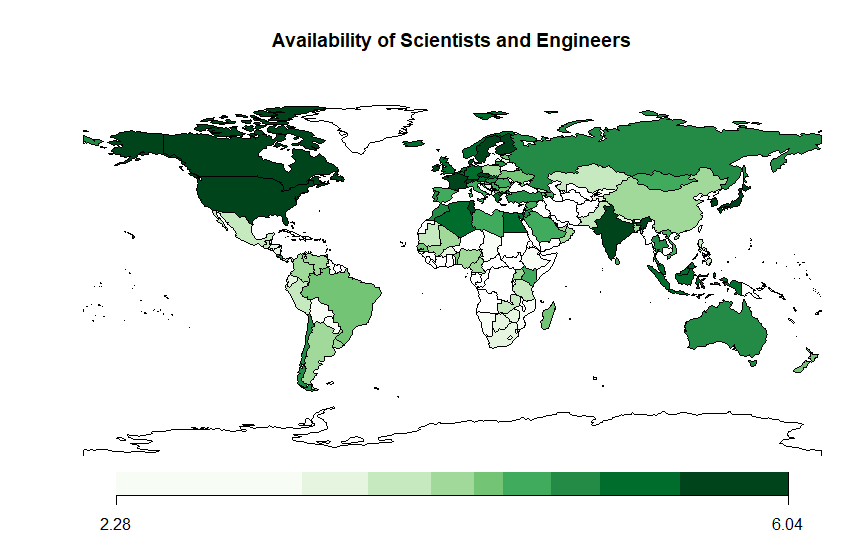
\includegraphics[scale = 0.7]{Part6_stem_avail.png}
    \caption{Availability of Scientists and Engineers Around the World Between 2017-2018}
\end{figure}

\begin{figure}[H]
    \centering
    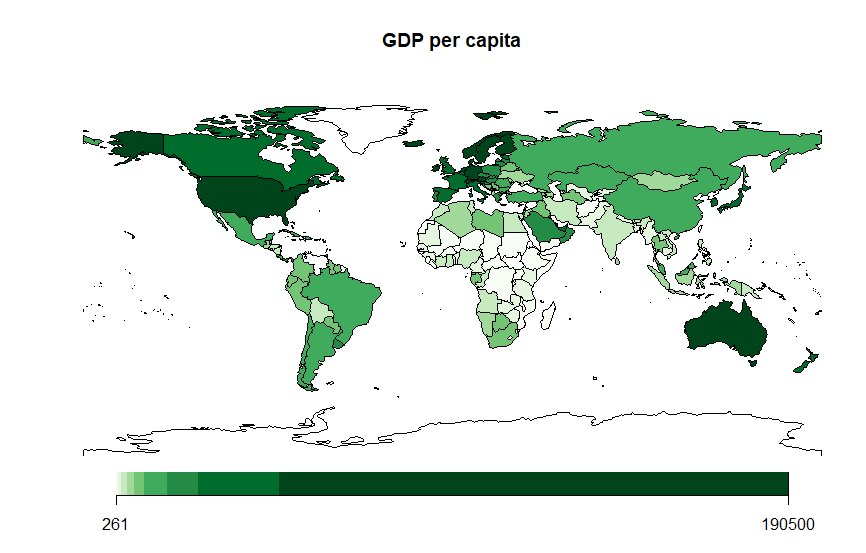
\includegraphics[scale = 0.7]{Part6_gdp_map.png}
    \caption{GDP per Capita Around the World in 2018}
\end{figure}
\noindent
In order to understand the correlation better, we plot a graph of the Availability of Scientists and Engineers against GDP per Capita in 2018, and run a linear regression model, as shown in Figures 33 and 34, respectively. The R-squared value of 0.3719 shows a low correlation, but is not statistically insignificant. We must understand that a high R-squared value only implies strong prediction, but does not rule out that data is good, and vice versa. Consider the negligible p-value, which suggests that the null hypothesis is false, and that the alternative hypothesis is true \cite{21}. This suggests that there is a significant correlation between the availability of scientists and engineers and GDP per capita of a country. However, as we have mentioned before, there are certain outliers to this correlation. \\
\\In general, it seems that more scientists and engineers means a faster modernization process within a country, as the talent required to develop technologies is readily available. Better technologies ensures efficiency in processes, resource gathering, transportation, internet, and other transportation means that allows a nation to create, build, and live. However, in countries like India where manufacturing is the prominent industry \cite{22}, the over-saturation of scientists and engineers does not contribute to significant economic growth. On the other hand, in China, where the economy is much more diverse, the relative lack of scientists and engineers does not significantly impede its economic growth. The correlation, therefore, exists because the availability of scientists and engineers remains an indicator of economic well-being, but is not applicable to all sociopolitical climates and economic conditions, especially in developing countries without mature infrastructure.
\\
\begin{figure}[H]
    \centering
    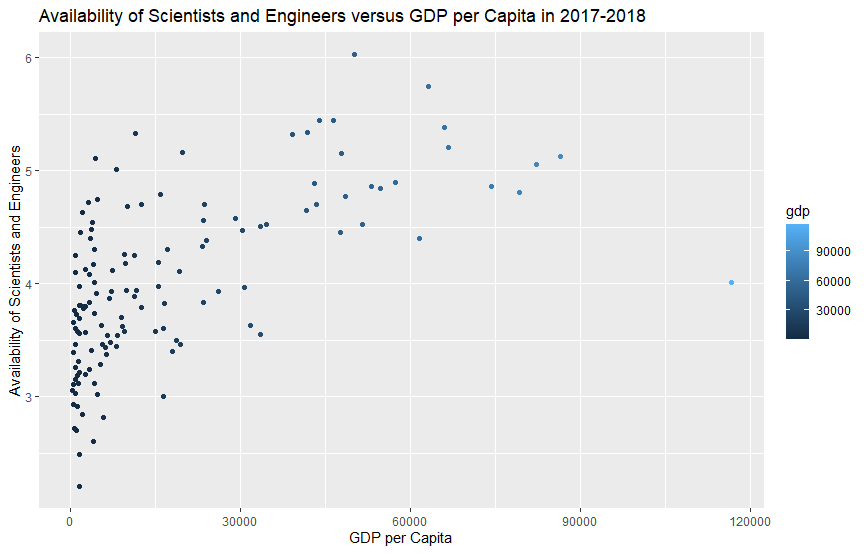
\includegraphics[scale = 0.7]{Part6_stem_avail_vs_gdp.png}
    \caption{Availability of Scientists and Engineers versus GDP per Capita Around the World in 2018}
\end{figure}

\begin{figure}[H]
    \centering
    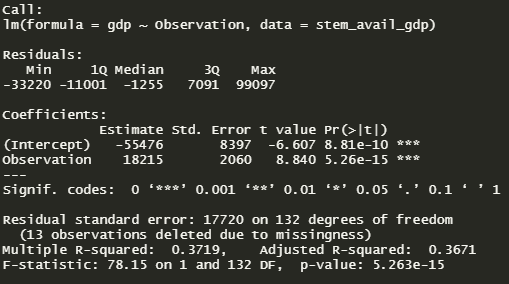
\includegraphics[scale = 0.7]{Part6_r^2.PNG}
    \caption{Statistical Correlation by Availability of Scientists and Engineers in 2018}
\end{figure}

\newpage

\section{Association of Gender Equality and Economic Growth}

Does GDP growth vary with gender equality? In order to understand this issue, we pull data from TCdata360's database \cite{2}, and find that the most recent gender equality data is from 2019. With this in mind, we plot the correlation between GDP growth and gender equality in 2019, as we can see in Figure 35. In Figure 36, we can see that there is almost no correlation with the data. However, as suggested by the p-value, we can see a line of best fit would suggest strong GDP growth in country's with poor gender equality indices. In fact, the largest GDP growths occurred in countries with a low gender equality index.

\begin{figure}[H]
    \centering
    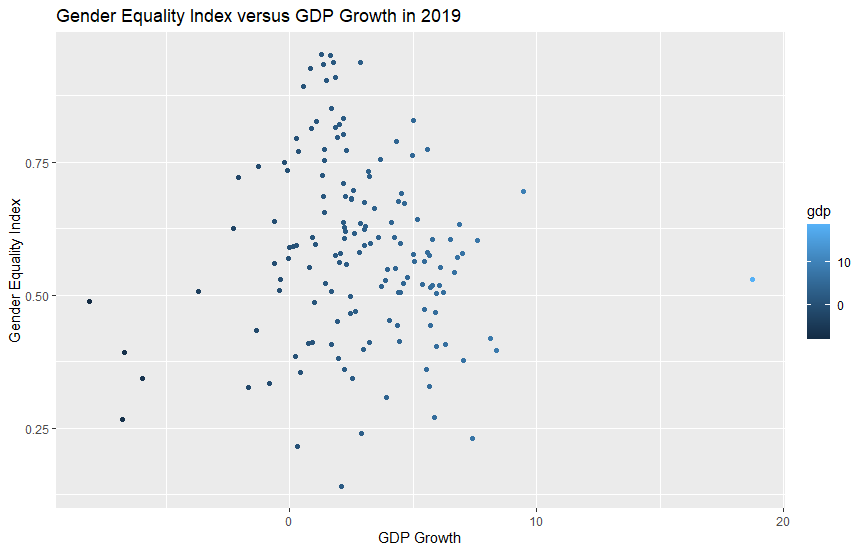
\includegraphics[scale = 0.5]{Part7_gender_growth.png}
    \caption{Gender Equality versus GDP Growth in 2019}
\end{figure}

\begin{figure}[H]
    \centering
    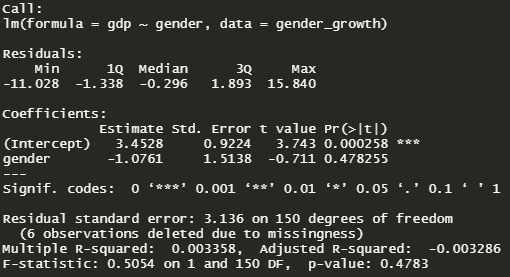
\includegraphics[scale = 0.7]{Part7_gender_growth_r^2.PNG}
    \caption{Statistical Correlation by Gender Equality in 2019}
\end{figure}

\noindent Intuitively, we associate gender equality with the end goal in workplace politics. However, this is often a luxury only developed nations can afford. In order to delve into this problem further, we now plot the correlation between GDP per capita and gender equality in 2019, and analyze its statistical properties, as we see in Figures 37 and 38, respectively. Immediately, we see a cluster or high GDP per capita nations that also exhibit high gender equality indices, as evidenced by a lower p-value and higher R-squared correlation. While the statistical significance for this relationship is yet to exist, it is a stronger relationship than that portrayed by GDP growth. Therefore, we can assume that economies tend to grow more quickly in nation's with a low gender equality index, but developed economies tend to exhibit higher gender equality. This is similar to the chicken and egg problem, where gender equality tends to come after the economy is developed.

\begin{figure}[H]
    \centering
    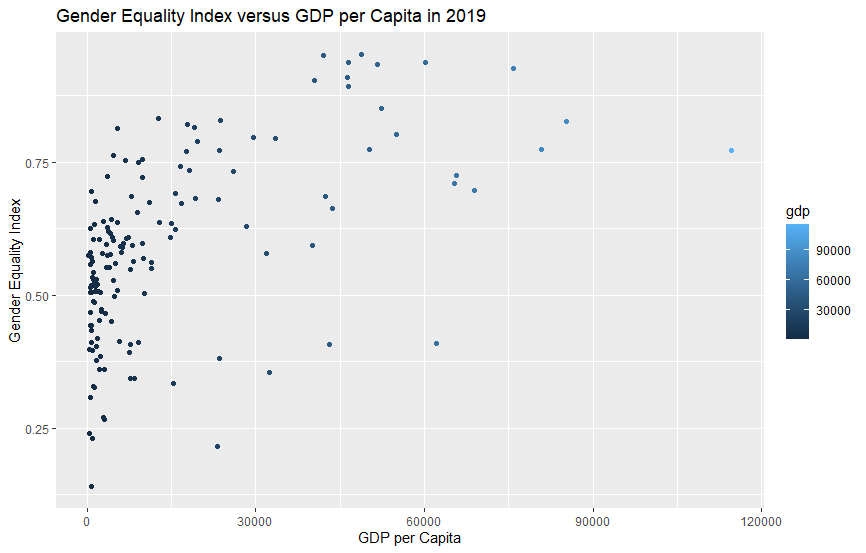
\includegraphics[scale = 0.5]{Part7_gender_capita.png}
    \caption{Gender Equality versus GDP per Capita in 2019}
\end{figure}

\begin{figure}[H]
    \centering
    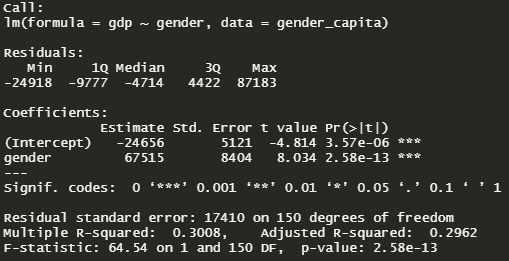
\includegraphics[scale = 0.65]{Part7_gender_capita_r^2.PNG}
    \caption{Statistical Correlation by Gender Equality in 2019}
\end{figure}

\noindent Regardless of the relationship between gender equality and GDP growth or GDP per capita, the top 5 countries that exhibited gender equality index growth between 2014-2019 were Canada, Singapore, Georgia, Azerbaijan, and Sri Lanka, as we can see in Figure 39.

\begin{figure}[H]
    \centering
    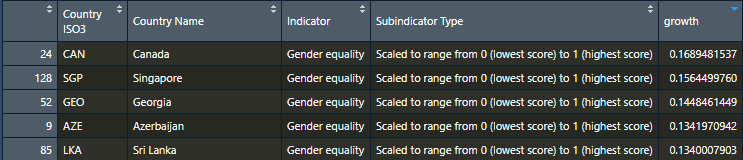
\includegraphics[scale = 0.7]{Part7_growth.PNG}
    \caption{Growth in Gender Equality Index between 2014-2019}
\end{figure}

\newpage

\begin{flushleft}
\bibliographystyle{IEEEtranN}
\begin{thebibliography}{9}
\bibitem{1} “International Money Transfer: Global Remittance with TranSwap,” International Money Transfer | Global Remittance with TranSwap. [Online]. Available: https://www.transwap.com/blog/us-dollar-how-it-became-the-global-currency. [Accessed: 29-Jan-2022]. 
\bibitem{2} “Innovation, Technology and Entrepreneurship: A data exploration,” Open Trade and Competitiveness Data. [Online]. Available: https://tcdata360.worldbank.org/. [Accessed: 29-Jan-2022]. 
\bibitem{3} “Northern Hemisphere,” Wikipedia, 04-Jan-2022. [Online]. Available: https://en.wikipedia.org/wiki/Northern\_Hemisphere\#cite\_note-8. [Accessed: 29-Jan-2022]. 
\bibitem{4} K. Wilkie, “Why colder countries are richer than Hot Nations,” Daily Mail Australia, 01-Jul-2020. [Online]. Available: https://www.dailymail.co.uk/news/article-8477297/Why-colder-countries-richer-hot-nations.html. [Accessed: 29-Jan-2022]. 
\bibitem{5} L. Ngo, “How to compare box plots,” BioTuring's Blog, 27-Sep-2020. [Online]. Available: https://blog.bioturing.com/2018/05/22/how-to-compare-box-plots/. [Accessed: 29-Jan-2022]. 
\bibitem{6} “Internet crossing borders: Boosting the internet in landlocked developing countries,” Growing the Internet, 06-Jan-2021. [Online]. Available: https://www.internetsociety.org/resources/doc/2017/lldcreport/. [Accessed: 29-Jan-2022]. 
\bibitem{7} P. Fox, “The global digital divide (article),” Khan Academy. [Online]. Available: https://www.khanacademy.org/computing/computers-and-internet/xcae6f4a7ff015e7d:the-internet/xcae6f4a7ff015e7d:the-digital-divide/a/the-global-digital-divide. [Accessed: 29-Jan-2022]. 
\bibitem{8} “Cambodian genocide,” Wikipedia, 26-Jan-2022. [Online]. Available: https://en.wikipedia.org/wiki/Cambodian\_genocide [Accessed: 29-Jan-2022]. 
\bibitem{9} “Civil War,” Encyclopædia Britannica. [Online]. Available: https://www.britannica.com/place/Cambodia/Civil-war. [Accessed: 29-Jan-2022]. 
\bibitem{10} “Rwanda Profile - Timeline,” BBC News, 17-Sep-2018. [Online]. Available: https://www.bbc.com/news/world-africa-14093322. [Accessed: 29-Jan-2022].
\bibitem{11} K. Thelwell, “Rising life expectancy in Africa,” The Borgen Project, 24-Apr-2019. [Online]. Available: https://borgenproject.org/rising-life-expectancy-in-africa/. [Accessed: 29-Jan-2022]. 
\bibitem{12} R. Ratcliffe, “Middle classes drive up life expectancy in sub-saharan africa,” The Guardian, 15-Sep-2018. [Online]. Available: https://www.theguardian.com/global-development/2018/sep/15/middle-classes-drive-up-life-expectancy-sub-saharan-africa-un-human-development-index-11-years. [Accessed: 29-Jan-2022]. 
\newpage\noindent
\bibitem{13} Z. Qiang, P. Kusek, V. Steenbergen, and B. Viney, “The road to recovery in Sub-Saharan africa: Capitalizing on transformative opportunities from shifting FDI patterns,” World Bank Blogs, 27-May-2021. [Online]. Available: https://blogs.worldbank.org/africacan/road-recovery-sub-saharan-africa-capitalizing-transformative-opportunities-shifting-fdi. [Accessed: 29-Jan-2022]. 
\bibitem{14} J. L. Dieleman, T. J. Bollyky, S. Crosby, and S. Kiernan, “Does healthier mean wealthier? measuring countries' economic performance during the pandemic: Think global health,” Council on Foreign Relations, 14-Jan-2021. [Online]. Available: https://www.thinkglobalhealth.org/article/does-healthier-mean-wealthier-measuring-countries-economic-performance-during-pandemic. [Accessed: 29-Jan-2022]. 
\bibitem{15} “Economic growth and life expectancy – do wealthier countries...,”  Euromonitor International, 14-Mar-2014. [Online]. Available: https://www.euromonitor.com/article/economic-growth-and-life-expectancy-do-wealthier-countries-live-longer. [Accessed: 29-Jan-2022]. 
\bibitem{16} A. Mahmoud, Class Lecture, Topic: "Week 2 - Understanding Poverty" APS420/APS1420, Faculty of Applied Science and Engineering, University of Toronto, Toronto, ON, Jan., 2022.
\bibitem{17} N. Dutta, R. S. Sobel, and S. Roy, “Entrepreneurship and political risk,” Journal of Entrepreneurship and Public Policy, 2013. [Online]. Available: https://ideas.repec.org/a/eme/jepppp/v2y2013i2p130-143.html. [Accessed: 29-Jan-2022]. 
\bibitem{18} C. Boyte-White, “How should a company be raising capital?,” Investopedia, 03-Nov-2021. [Online]. Available: https://www.investopedia.com/ask/answers/032515/what-are-different-ways-corporations-can-raise-capital.asp. [Accessed: 29-Jan-2022]. 
\bibitem{19} M. Riordan, “No monopoly on Innovation,” Harvard Business Review, 01-Aug-2014. [Online]. Available: https://hbr.org/2005/12/no-monopoly-on-innovation [Accessed: 29-Jan-2022]. 
\bibitem{20} History.com Editors, “Stock market crash of 1929,” History.com, 10-May-2010. [Online]. Available: https://www.history.com/topics/great-depression/1929-stock-market-crash. [Accessed: 29-Jan-2022]. 
\bibitem{21} S. A. McLeod, “What a p-value tells you about statistical significance.,” Simply Psychology, 20-May-2019. [Online]. Available: www.simplypsychology.org/p-value.html. [Accessed: 29-Jan-2022]. 
\bibitem{22} “Contribution by some Major Industries,” Toppr. [Online]. Available: https://www.toppr.com/guides/fundamentals-of-economics-cma/indian-economy/contribution-by-some-major-industries/. [Accessed: 29-Jan-2022]. 
\end{thebibliography}
\end{flushleft}

\newpage

\section{Appendix A}

\lstset{
  breaklines=true,
}
\lstinputlisting[language=R]{assignment_1.R}


\end{document}